\section{Riadkovo-stĺpcový aditívny model s dvoma typmi ošetrení}
\label{my model}

Cieľom tejto práce je skúmať experiment reprezentovaný binárnou maticou.
Možná reprezentácia nášho modelu pri matici rozmeru $m \times n$ je takáto:

Uvažujeme model s dvomi kvalitatívnymi faktormi $A$ a $B$, 
pričom faktor $A$ má $m$ úrovní a faktor $B$ $n$ úrovní. 
Pre každú kombináciu faktorov experimentátor zvolí jedno z dvojice ošetrení (angl. treatment).
Budeme uvažovať len aditívny model bez interakcií.

Napríklad faktor $A$ môže označovať dobrovoľníka (t.j. máme $m$ dobrovoľníkov) 
a faktor $B$ účinnú látku, ktorú nazveme liečivo (t.j. máme $n$ liečiv). 
Ošetrenie $0$ reprezentuje podanie liečiva orálnym spôsobom a ošetrenie $1$ vnútrožilne).
Účinok, ktorý po čase nameriame na dobrovoľníkovi, 
závisí aditívne od efektu samotného dobrovoľníka (jeho predispozícií), 
efektu liečiva a efektu ošetrenia. 
Všetky tieto efekty uvažujeme ako neznáme parametere modelu.

Návrh teda možno reprezentovať binárnou maticou 
(alebo bipartitným grafom, čo opíšeme neskoršie vnašej práci).

Cieľom experimentu je odhadnúť rozdiel medzi dvoma efektmi (treamentami).
Cieľom hľadania optimálneho modelu je nájsť taký návrh, pri ktorom
rozptyl Gauss-Markovovho odhadu rozdielu medzi efektmi dvojice ošetrení (t.j. odhadu kontrastu ošetrení) bude čo najmenší.
(Použijeme pri tom Gaussovu-Markovovu vetu z predošlej kapitoly.)

Pre maticu typu $m \times n$ dostaneme teda $mn$ vzťahov tvaru:

\begin{center}
$
y_{ij} = a_i + b_j + t + e_{ij}
$
\end{center}

$i = 1, \ldots, m$; $j = 1, \ldots, n$; $t$ je $t_0$ alebo $t_1$ podľa hodnoty na $ij$-tej pozícii matice a $e_{ij}$ je chyba.
Budeme odhadovať rozdiel medzi $t_0$ a $t_1$.

Z návrhu modelu v podobe binárnej matice tvaru $m \times n$ vytvoríme lineárny regresný model
s maticou tvaru $mn \times (m + n + 2)$, pretože máme $mn$ meraní závislých od $m + n + 2$ premenných.

Príklad:

Maticu návrhu experimentu

\begin{align}
\label{model matrix}
\begin{bmatrix}
1 & 0 & 1 \\
0 & 1 & 0 \\
1 & 0 & 1
\end{bmatrix}
\end{align}

prepíšeme ako:

\begin{align}
\label{linear regression matrix}
\begin{bmatrix}
1 & 0 & 0 & 1 & 0 & 0 & 1 & 0 \\
1 & 0 & 0 & 0 & 1 & 0 & 0 & 1 \\
1 & 0 & 0 & 0 & 0 & 1 & 1 & 0 \\
0 & 1 & 0 & 1 & 0 & 0 & 0 & 1 \\
0 & 1 & 0 & 0 & 1 & 0 & 1 & 0 \\
0 & 1 & 0 & 0 & 0 & 1 & 0 & 1 \\
0 & 0 & 1 & 1 & 0 & 0 & 1 & 0 \\
0 & 0 & 1 & 0 & 1 & 0 & 0 & 1 \\
0 & 0 & 1 & 0 & 0 & 1 & 1 & 0
\end{bmatrix}
\end{align}

Ako presne sme pri generovaní matice postupovali?
Každý riadok reprezentuje jednu z hodnôt v matici (\ref{model matrix}), preto máme dokopy $3 \times 3 = 9$ riadkov.
Prvé tri stĺpce reprezentujú riadok, v ktorom sa hodnota nachádza, ďalšie tri reprezentujú stĺpec.
Vo všeocenosti $ij$-tu pozíciu matice typu $m \times n$ reprezentuje riadok,
ktorý má jednotky na $i$-tej a $(m + j)$-tej pozícii.
Posledné dva stĺpce sú určené tým, či je hodnota $0$ alebo $1$.

Označme vo všeobecnosti maticu modelu (\ref{model matrix}) $B$ a maticu lineárneho zobrazenia (\ref{linear regression matrix}) $X$. 
Predpokladáme lineárne vzťahy, preto dostávame lineárnu regresiu

\begin{center}
$
y = X b + e
$
\end{center}

kde $y$ je vektor dát nameraných v experimente, $b$ je vektor neznámych koeficientov a 
$e = (e_{11}, e_{12}, e_{13}, \ldots, e_{m1}, \dots, e_{mn})^T$ je vektor chýb merania. 
Uvedomme si, že v našej práci nebudeme pracovať s konkrétnym vektorom $y$; 
snažíme sa totiž navrhnúť maticu modelu $B$ (a z nej vyplývajúcu maticu $X$) ešte pred tým, než experiment vykonáme.

Naším cieľom teraz bude odhadnúť rozdiel medzi efektmi $t_0$ a $t_1$, resp. zistiť, 
aká môže byť disperzia tohto odhadu pri danej matici návrhu $B$. 
Modely, pre ktoré bude možná disperzia najmenšia, budeme považovať za optimálne.

V danej lineárnej regresii $y = X b + e$ teda nebudeme odhadovať celý vektor $b$, 
ale len jeho lineárnu kombináciu $h^T b$, kde $h$ je vektor rozmeru $m + n + 2$, 
ktorý má na $m + n$ miestach $0$ a na zvyšných dvoch miestach $+1$ a $-1$, ktoré zodpovedajú efektom $t_0$ a $t_1$. 
Z algoritmu, ktorým sme z matice návrhu $B$ vytvorili maticu lineárnej regresie $X$, 
vyplýva, že vektor $h$ má tvar $(0, 0, 0, \ldots, +1, -1)^T$.

Na zistenie, či $h^T b$ je odhadnuteľné, použijeme vetu (\ref{veta1}), 
a na následné nájdenie minimálneho rozptylu Gauss-Markovovho odhadu rozdielu medzi efektmi 
použijeme Gaussovu-Markovovu vetu (\ref{gauss-markov}).

\subsection{Odhadnuteľnosť $h^T b$}

Pokúsime sa preskúmať, kedy matica návrhu umožňuje odhadnuteľnosť hodnoty $h^T b$ pre vyššie spomenuté $h$. 
Situáciu preskúmame do rozmeru $4 \times 5$ a na základe našich zistení vyslovíme hypotézu pre všeobecný prípad $m \times n$.

Postupovať budeme nasledovne: vyberieme si malý rozmer a pre všetky matice daného rozmeru zistíme, 
či $h^T b$ bude alebo nebude odhadnuteľné, a to nasledovným spôsobom. 
Z danej matice návrhu $B$ vytvoríme maticu lineárnej regresie $X$ spôsobom spomenutým vyššie. 
Hodnota $h^T b$ bude na základe vety (\ref{veta1}) odhadnuteľná práve vtedy, 
keď vektor $h = (0, 0, 0, \ldots, +1, -1)^T$ patrí do stĺpcového priestoru matice $X^T X$.

Označme $M = X^T X$, túto maticu budeme nazývať informačnou maticou. 
Ak $h$ patrí do stĺpcového priestoru $M$, potom existuje taký vektor $v$, že $M v = h$. 
Na základe vety (\ref{veta3}) vieme, že ak toto riešenie existuje, tak sa rovná $M^- h$, pričom zvolená $g$-inverzia môže byť ľubovoľná.
Preto na zistenie, či $h$ patrí do stĺpcového priestoru $M = X^T X$ stačí overiť platnosť rovnosti $M(M^- h) = h$. 

Demonštrujme algoritmus na maticiach rozmeru $3 \times 3$. Existuje $2^9 = 512$ binárnych matíc typu $3 \times 3$, 
a keď sme na nich rozbehli daný algoritmus, dospeli sme k zisteniu, že pri $12$ z nich hodnota $h^T b$ NIE JE odhadnuteľná.
To znamená, že optimálne matice návrhu budeme hľadať v zvyšných $500$ maticiach.

Ako vyzerajú matice, pri ktorých $h^T b$ nie je odhadnuteľné? Zoznam všetkých sa nachádza v Prílohe A, tu uvedieme $3$ z nich:

\begin{center}
$
\begin{bmatrix}
1 & 1 & 1 \\
0 & 0 & 0 \\
1 & 1 & 1 \\
\end{bmatrix}
$, 
$
\begin{bmatrix}
0 & 0 & 1 \\
0 & 0 & 1 \\
0 & 0 & 1 \\
\end{bmatrix}
$, 
$
\begin{bmatrix}
0 & 0 & 0 \\
0 & 0 & 0 \\
0 & 0 & 0 \\
\end{bmatrix}
$
\end{center}

Týmto spôsobom sme pri našom výskume získali zoznam matíc, pri ktorých $h^T b$ nie je odhadnuteľné, až do rozmeru $4 \times 5$.
Zoznam všetkých sa nachádza v GitHub repozitári spomenutom v úvode. 
Na základe podobnosti matíc daného typu sme prišli s nasledovnou hypotézou.

\begin{prop}
\label{statement 1}
$h^T b$ je odhadnuteľné práve vtedy, keď v matici návrhu $B$ existuje aspoň jeden riadok a aspoň jeden stĺpec taký,
ktorý má aspoň jednu $0$ a aspoň jednu $1$.
\end{prop}

\begin{dokaz}
Na základe vety (\ref{veta1}) vieme, že $h^T b$ je odhadnuteľné práve vtedy, keď $h \in \mathcal{M}(X^T)$
(keď $h$ patrí do riadkového priestoru $X$),
preto s danými podmienkami môžeme pracovať ekvivalentne.

$\boxed{\implies}$ Nech $h = (0, \ldots, +1, -1) \in \mathcal{M}(X^T)$. Použijeme dôkaz sporom. 
Nech v matici $B$ typu $m \times n$ neexistuje taký riadok, ktorý má aspoň jednu $0$ a aspoň jednu $1$,
t. j všetky riadky obsahujú buď samé $0$ alebo samé $1$.
Ako vyzerá matica $X$?

Pozrime sa na riadky matice $X$ zodpovedajúce prvému riadku matice $B$.
Sú to práve tie riadky, ktoré majú na prvej pozícii $1$, pričom si uvedomme, že všetky ostatné riadky majú na prvej pozícii $0$.

% TODO
\begin{center}
$
x_1 = (1, 0, \ldots, 1, 0, \ldots, 0, 1, 0)
$,
\end{center}
\begin{center}
$
x_2 = (1, 0, \ldots, 0, 1, \ldots, 0, 1, 0)
$,
\end{center}
\begin{center}
$\vdots$
\end{center}
\begin{center}
$
x_n = (1, 0, \ldots, 0, 0, \ldots, 1, 1, 0)
$
\end{center}

Keďže $h \in \mathcal{M}(X^T)$, existuje taká lineárna kombinácia riadkov $X$, ktorá dokopy dáva vektor $h$.
Aké môžu mať v tejto lineárnej kombinácii zastúpenie riadky $x_1$, ..., $x_n$?
Označme postupne $a_1$, ..., $a_n$ koeficienty vektorov $x_1$, ..., $x_n$ v lineárnej kombinácii riadkov $X$, ktorá dáva vektor $h$.
Keďže $x_1$, ..., $x_n$ sú jediné riadky matice $X$ s $1$ na prvej pozícii a vektor $h$ má na prvej pozícii $0$,
musí platiť $\sum_{i = 1}^n a_i = 0$.

Z predpokladu, že každý z riadkov matice $B$ obsahuje buď samé $0$ alebo samé $1$, vyplýva,
že každý z vektorov $x_1$, ..., $x_n$ má rovnaké posledné dve hodnoty, a to buď $(0, 1)$ alebo $(1, 0)$.
Z toho spolu s rovnosťou $\sum_{i = 1}^n a_i = 0$ vyplýva, že lineárna kombinácia $\sum_{i = 1}^n a_i x_i$
bude mať na posledných dvoch miestach hodnoty $(0, 0)$, a teda nijako "neprispeje" do vektoru $h$.
Vektor $h$ teda nemožno napísať ako lineárnu kombináciu riadkov $X$, čo je podmienka odhadnuteľnosti.

Analogicky môžeme postupovať pre všetky riadky matice $B$.
Týmto spôsobom pokryjeme všetky riadky matice $X$, vďaka čomu dospejeme k záveru,
že z riadkov $X$ nie je možné lineárnou kombináciou zostrojiť vektor $h$.
To nám dáva spor s predpokladom $h \in \mathcal{M}(X^T)$.
Preto nemôže platiť, že všetky riadky matice $B$ obsahujú buď samé $0$ alebo samé $1$,
a platí opačné tvdenie, t.j v $B$ existuje aspoň jeden riadok taký, ktorý obsahuje $0$ aj $1$.

Rovnakou úvahou pre stĺpce $B$ dospejeme k záveru,
že $B$ musí takisto obsahovať aspoň jeden stĺpec obsahujúci $0$ aj $1$.

$\boxed{\impliedby}$ Nech matica $B$ je taká, že existuje aspoň jeden riadok a aspoň jeden stĺpec také, že majú $0$ aj $1$.
Zostrojíme takú lineárnu kombináciu riadkov $X$, ktorá sa bude rovnať $h$.

Nech riadok, ktorý má $0$ aj $1$, je $i$-ty v poradí a stĺpec s rovnakou vlastnosťou je $j$-ty v poradí.
Bez ujmy na všeobecnosti, nech na $ij$-tom mieste matice $B$ sa nachádza $0$, teda $B_{ij} = 0$.

Potom v $i$-tom riadku $B$ sa určite nachádza hodnota $B_{ik} = 1$ a v $j$-tom stĺpci sa nachádza hodnota $B_{lj} = 1$,
pričom, samozrejme, $k \neq j$ a $l \neq i$.
Označme $x_{ij}, x_{ik}, x_{lj}, x_{lk}$ riadky matice $X$ prislúchajúce prvkom $B_{ij}, B_{ik}, B_{lj}, B_{lk}$ matice $B$. Potom:

\begin{center}
$
x_{ij} - x_{ik} - x_{lj} + x_{lk} = (0, 0, 0, \ldots, 0, N_1, N_2)
$
\end{center}
je vektor, ktorý má na prvých $m + n$ miestach $0$, a na posledných dvoch hodnoty $N_1$ a $N_2$, ktoré zatiaľ necháme bokom.
Prečo má daný vektor na prvých $m + n$ miestach $0$?
Vo všeobecnosti má riadok $x_{rs}$ matice $X$ prislúchajúci prvku $B_{rs}$ matice $B$ na prvých $m + n$ miestach dve $1$,
jednu prislúchajúcu riadku, druhú stĺpcu matice $B$. Konkrétne, riadok $x_{rs}$ má $1$ na $r$-tom mieste a $(m + s)$-tom mieste.

Súčet $x_{ij} + x_{lk}$ má teda štyri jednotky na miestach $i, j, m + j, m + k$.
Súčet $x_{ik} + x_{lj}$ má jednotky na tých istých miestach, 
preto $x_{ij} - x_{ik} - x_{lj} + x_{lk} = x_{ij} + x_{lk} - (x_{ik} + x_{lj})$ má na prvých $m + n$ miestach $0$.

Takto to vyzerá, keď zanedbáme stĺpce so samými nulami:
\[
\begin{split}
+(1, 0, 1, 0) \\
-(1, 0, 0, 1) \\
-(0, 1, 1, 0) \\
+(0, 1, 0, 1) \\
=(0, 0, 0, 0) \\
\end{split}
\]

Ako vyzerá chvost $(N_1, N_2)$? Keďže $B_{ij} = 0$ a $B_{ik} = B_{lj} = 1$,
výraz $x_{ij} - x_{ik} - x_{lj}$ nám vytvorí chvost $(1, -2)$ (prípadne $(-2, 1)$, na tom ale nezáleží).
Potom na základe toho, či na mieste $B_{lk}$ matice návrhu bola $0$ alebo $1$,
nám výraz $x_{ij} - x_{ik} - x_{lj} + x_{lk}$ dá na posledných dvoch miestach $(2, -2)$ alebo $(1, -1)$.
Vo všetkých prípadoch vektor $h$ dostaneme ihneď, prípadne po prenásobení konštantou.
Našli sme teda lineárnu kombináciu riadkov $X$, ktorá nám dala vektor $h$, preto $h \in \mathcal{M}(X^T)$. $\square$

\end{dokaz}

\subsection{Ekvivalencie binárnych matíc}

Pre rozmer $m \times n$ existuje $2^{mn}$ binárnych matíc, čo je obrovské číslo už pre malé hodnoty $m$ a $n$.
(Napríklad už pre rozmer $5 \times 5$ máme viac než milión matíc.)
Pre skúmanie špecifík jednotlivých matíc je výhodné uvedomiť si niektoré očividné ekvivalencie medzi maticami, 
čo nám môže výrazne zredukovať počet matíc, s ktorými pracujeme,
 a v konečnom dôsledku nám to umožní pracovať spôsobom “brute force” do väčšieho rozmeru.

\begin{hypoteza}

Matice, ktoré možno spermutovať jednu na druhú riadkovými a stĺpcovými permutáciami, sú ekvivalentné v zmysle, 
že majú rovnakú hodnotu minimálneho rozptylu Gaussovho-Markovho rozdielu medzi dvoma efektmi.

\end{hypoteza}

Hypotézu uvádzame bez matematického dôkazu, ukážeme však, že ak naša interpretácia modelu reprezentovaného binárnou maticou je správna,
hypotéza musí platíť. Model sme interpretovali ako zoznam trojíc pacient, lekár, spôsob prijatia lieku, 
pričom pacienti zodpovedali riadkom, lekári stĺpcom, a spôsob prijatia lieku hodnotám v matici. 
Uvedomme si, že o lekároch ani pacientoch pri výpočte rozptylu nič nevieme. 
Permutáciám riadkov a stĺpcov preto zodpovedá akési „prelabelovanie“ jednotlivých lekárov a pacientov, 
vôbec to ale nezmení štruktúru experimentu. Pripomeňme si, že rozptyl Gaussovho-Markovho rozdielu medzi efektmi 
počítame pred vykonaním experimentu a nameraním dát.

Táto jediná ekvivalencia nám výrazne zredukuje počet matíc, s ktorými musíme počítať. 
V tabuľke uvádzame počet neekvivalentných tried pre štvorcové rozmery až do $6 \times 6$.

\begin{center}
\begin{tabular}{ |c|c|c|c|c|c|c| }
  \hline
  Rozmer & $1 \times 1$ & $2 \times 2$ & $3 \times 3$ & $4 \times 4$ & $5 \times 5$ & $6 \times 6$ \\ \hline
  Počet binárnych matíc & 2 & 16 & 512 & 65 536 & 33 554 432 & 68 719 476 736 \\ \hline
  Počet neekvivalentných tried & 2 & 7 & 36 & 317 & 5 624 & 251 610 \\ \hline
\end{tabular}
\end{center}

\subsection{Optimálnosť návrhu modelu}

Teraz sa pokúsime nájsť modely, ktoré pre nás budú v určitom zmysle optimálne. 
Najprv ale definujme, čo presne optimalita modelu znamená.

\begin{defin}
\label{optimal matrix definition}
Binárnu maticu $B$ návrhu modelu, $B \in \mathbb{R}^{m \times n}$, nazývame optimálnou, 
ak pre všetky binárne matice $C \in \mathbb{R}^{m \times n}$ platí:

\begin{center}
\label{optimal matrix}
$h^T M_{B}^- h \leq h^T M_{C}^- h$
\end{center}
kde $h = (0, 0,\ldots , +1, -1)$ je vektor zodpovedajú lineárnej kombinácii dvoch efektov, 
$M_B$ a $M_C$ sú informačné matice prislúchajúce návrhom $B$, $C$ a $M_{B}^-$, $M_{C}^-$ sú ich ľubovolné pseudoinverzie.

\end{defin}

Nájsť optimálne matice v zmysle definície (\ref{optimal matrix}) je cieľom tejto práce. 
Podobne ako pri skúmaní, či hodnotu $h^T b$ vôbec budeme môcť odhadnúť, 
preskúmame najprv matice malého rozmeru a na základe výsledkov vyslovíme hypotézu pre všeobecný rozmer.

Postupovať budeme nasledovne: zoberieme si malý rozmer a pre všetky binárne matice tohto rozmeru spočítame hodnotu $h^T M^- h$, 
pokiaľ je to možné (viď tvrdenie (\ref{statement 1})). Z množiny týchto hodnôt vyberieme minimum. 
Optimálne návrhy budú tie, ktorých prislúchajúca hodnota bude práve toto minimum.

Optimálne návrhy sme určili do rozmeru $6 \times 5$, tu sú niektoré z nich pre štvorcové rozmery:

\begin{center}
$
\begin{bmatrix}
0 & 1 & 1 \\ 
1 & 0 & 1 \\ 
1 & 1 & 0 \\ 
\end{bmatrix}
$, 
$
\begin{bmatrix}
0 & 0 & 1 & 1 \\
0 & 0 & 1 & 1 \\
1 & 1 & 0 & 0 \\
1 & 1 & 0 & 0 \\
\end{bmatrix}
$, 
$
\begin{bmatrix}
0 & 0 & 1 & 1 & 0 \\
0 & 1 & 0 & 1 & 0 \\
0 & 1 & 1 & 0 & 0 \\
1 & 0 & 0 & 0 & 1 \\
1 & 0 & 0 & 0 & 1 \\
\end{bmatrix}
$
\end{center}

Ďalšie matice sa nachádzajú v prílohe B. Na základe týchto návrhov sme pre štvorcové matice prišli s nasledovnou hypotézou.

\begin{hypoteza}
\label{hypoteza1}
(pre štvorcové matice)

Binárna matica návrhu $B$ rozmeru $2k \times 2k$ je optimálna v zmysle definície (\ref{optimal matrix}) práve vtedy, 
keď má v každom riadku a v každom stĺpci práve $k$ jednotiek (a práve $k$ núl).

Binárna matica návrhu $B$ rozmeru $(2k + 1) \times (2k + 1)$ je optimálna práve vtedy, 
keď všetky jej riadky aj stĺpce majú rovnaký počet jednotiek, a ten počet je buď $k$ alebo $k + 1$.
\end{hypoteza}

Ako to vyzerá pre matice iného, ako štvorcového rozmeru? 
Kľúčový je pomer jednotiek a núl v matici návrhu. 
Všimnime si, že pri štvorcových rozmeroch v predošlej hypotéze je v prípade párneho rozmeru rovnaký počet jednotiek a núl, 
no v prípade nepárneho rozmeru pomer nielenže nie je pol na pol (čo ani nemôže byť), 
ale dokonca k tomuto pomeru ani nie je tak blízko, ako by mohol byť. 
Napríklad pri rozmere $5 \times 5$ by sme mohli očakávať, že pomer jednotiek a núl v optimálnom návrhu bude $13:12$, 
ale podľa hypotézy je to $15:10$. Skutočnosť, že $5$ delí $10$ aj $15$, nie je náhodná, 
a bude zohrávať kľúčovú rolu pri hypotéze o návrhoch iných ako štvorcových rozmerov.

\begin{hypoteza}
\label{hypoteza2}
(pre neštvorcové matice)

Postačujúcou podmienkou optimality pre rozmer $2k \times 2l$ je, ak má matica práve $2kl$ jednotiek a $2kl$ núl, 
pričom v každom z $2k$ riadkov je $l$ jednotiek a $l$ núl a v každom z $2l$ stĺpcov je práve $k$ jednotiek a $k$ núl.

Postačujúcou podmienkou optimality pre rozmer $2k \times 2l + 1$ je, ak má matica práve $(2l + 1)k$ jednotiek a $(2l + 1)k$ núl, 
pričom v každom z $2l + 1$ stĺpcov je práve $k$ jednotiek a $k$ núl, v $k$ riadkoch je $l + 1$ jednotiek a $l$ núl 
a v $k$ zvyšných riadkoch je $l$ jednotiek a $l + 1$ núl.

Ďalej nech bez ujmy na všeobecnosti $k < l$.

Postačujúcou podmienkou optimality pre rozmer $2k + 1 \times 2l + 1$ je, 
ak má matica $(l + 1)(2k + 1)$ jednotiek a $l(2k + 1)$ núl (alebo naopak), 
pričom v každom z $2k + 1$ riadkov je práve $l + 1$ jednotiek a $l$ núl, v $l + k + 1$ stĺpcoch je práve $k + 1$
jednotiek a v $l - k$ stĺpcoch je práve $k$ jednotiek.
\end{hypoteza}

\begin{com}
Podmienky nie sú nutné, pretože napr. pri rozmere $3 \times 6$ sme našli optimálne matice s pomerom jednotiek a núl
nielen $9:9$ (spĺňajúce hypotézu), ale aj $6:12$, čo naznačuje, 
že v niektorých prípadoch matice pokryté hypotézou nie sú všetky optimálne matice daného rozmeru. 
Hypotéza je napriek tomu cenná, pretože pre prax nám poskytuje mechanizmus, ako vytvoriť optimálny návrh experimentu.
\end{com}

Niektoré z optimálnych návrhov pre neštvorcové rozmery:

\begin{center}
$
\begin{bmatrix}
0 & 0 & 1 & 1 \\
0 & 0 & 1 & 1 \\
1 & 1 & 0 & 0 \\
\end{bmatrix}
$,
$
\begin{bmatrix}
0 & 0 & 0 & 0 & 1 & 1 & 1 \\
0 & 1 & 1 & 1 & 0 & 0 & 0 \\
1 & 0 & 0 & 1 & 0 & 0 & 1 \\
\end{bmatrix}
$,
$
\begin{bmatrix}
0 & 0 & 1 & 1 & 1 \\ 
0 & 1 & 0 & 0 & 1 \\ 
0 & 1 & 0 & 1 & 0 \\ 
1 & 0 & 0 & 0 & 1 \\ 
1 & 0 & 1 & 1 & 0 \\ 
1 & 1 & 1 & 0 & 0 \\ 
\end{bmatrix}
$
\end{center}

Niektoré z optimálnych návrhov pre rozmer $3 \times 6$:

\begin{center}
$
\begin{bmatrix}
0 & 0 & 0 & 0 & 1 & 1 \\
0 & 0 & 1 & 1 & 0 & 0 \\
1 & 1 & 0 & 0 & 0 & 0 \\
\end{bmatrix}
$,
$
\begin{bmatrix}
0 & 0 & 0 & 1 & 1 & 1 \\
0 & 0 & 0 & 1 & 1 & 1 \\
1 & 1 & 1 & 0 & 0 & 0 \\
\end{bmatrix}
$,
$
\begin{bmatrix}
0 & 0 & 1 & 1 & 1 & 1 \\
1 & 1 & 0 & 0 & 1 & 1 \\
1 & 1 & 1 & 1 & 0 & 0 \\
\end{bmatrix}
$
\end{center}

\subsection{Hodnota minimálneho rozptylu}

Ako závisí hodnota (minimálna) Gaussovho-Markovovho rozptylu od rozmeru matice návrhu? 
Ukážeme, že minimálny rozptyl má so stúpajúcim rozmerom klesajúcu tendenciu. 
(Čo, napokon, dáva zmysel, pretože väčší rozdiel nám ponúka viac dát na určenie rozdielu medzi dvoma efektmi.)

Hodnoty pre jednotlivé rozmery určíme tak, že pre každý rozmer zoberieme jednu maticu optimálnu 
v zmysle definície (\ref{optimal matrix definition}) a určíme ju pre ňu.

Matice vytvoríme tak, aby spĺňali hypotézu (\ref{hypoteza1}), a to nasledovne.

Pre párny rozmer $2k \times 2k$ rozdelíme maticu na $4$ bloky $k \times k$, 
z nich ľavý horný a pravý dolný budú samé jednotky, zvyšné dva samé nuly. 
Pre nepárny rozmer $(2k + 1) \times (2k + 1)$ budú ľavý horný blok $k \times k$ tvoriť samé jednotky 
a pravý dolný blok $(k + 1) \times (k + 1)$ bude identita, v ktorej sa zamenili jednotky a nuly.

Názorný príklad, ako to vyzerá pre rozmery $6 \times 6$ a $7 \times 7$:

\begin{center}
$
\begin{bmatrix}
1 & 1 & 1 & 0 & 0 & 0 \\
1 & 1 & 1 & 0 & 0 & 0 \\
1 & 1 & 1 & 0 & 0 & 0 \\
0 & 0 & 0 & 1 & 1 & 1 \\
0 & 0 & 0 & 1 & 1 & 1 \\
0 & 0 & 0 & 1 & 1 & 1 \\
\end{bmatrix}
$,
$
\begin{bmatrix}
1 & 1 & 1 & 0 & 0 & 0 & 0 \\
1 & 1 & 1 & 0 & 0 & 0 & 0 \\
1 & 1 & 1 & 0 & 0 & 0 & 0 \\
0 & 0 & 0 & 0 & 1 & 1 & 1 \\
0 & 0 & 0 & 1 & 0 & 1 & 1 \\
0 & 0 & 0 & 1 & 1 & 0 & 1 \\
0 & 0 & 0 & 1 & 1 & 1 & 0 \\
\end{bmatrix}
$
\end{center}

V tabuľke a grafe sú znázornené hodnoty rozptylu do rozmeru $15 \times 15$.

\begin{center}
\begin{tabular}{ |c|c|}
  \hline
  Rozmer & Minimálna hodnota rozptylu \\ \hline
  $2 \times 2$ & 1 \\ \hline
  $3 \times 3$ & 0.5 \\ \hline
  $4 \times 4$ & 0.25 \\ \hline
  $5 \times 5$ & 0.167 \\ \hline
  $6 \times 6$ & 0.111 \\ \hline
  $7 \times 7$ & 0.083 \\ \hline
  $8 \times 8$ & 0.063 \\ \hline
  $9 \times 9$ & 0.05 \\ \hline
  $10 \times 10$ & 0.04 \\ \hline
  $11 \times 11$ & 0.033 \\ \hline
  $12 \times 12$ & 0.028 \\ \hline
  $13 \times 13$ & 0.024 \\ \hline
  $14 \times 14$ & 0.02 \\ \hline
  $15 \times 15$ & 0.018 \\ \hline
\end{tabular}
\end{center}

\begin{figure}[!h]
  \centering
  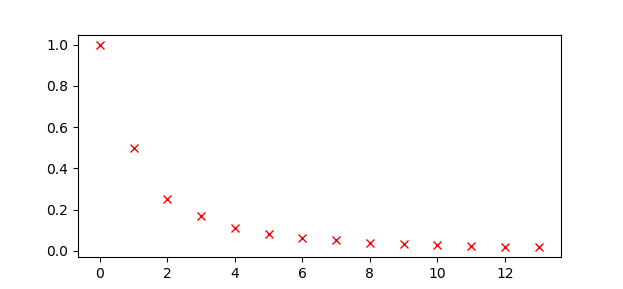
\includegraphics{minimalny_rozptyl.png}
\end{figure}
